\documentclass{beamer}
\mode<presentation>
{
  \usetheme{Warsaw}      % or try Darmstadt, Madrid, Warsaw, ...
  \usecolortheme{beaver} % or try albatross, beaver, crane, ...
  \usefonttheme{default}  % or try serif, structurebold, ...
  \setbeamertemplate{navigation symbols}{}
  \setbeamertemplate{caption}[numbered]
  \setbeamertemplate{footline}[frame number]
}


\usepackage[english]{babel}
\usepackage{chronology}
\usepackage[utf8]{inputenc}
\usepackage{pgfpages}
\usepackage{algorithm}
\usepackage{color}
\usepackage{verbatim}
\usepackage[noend]{algorithmic}
\usepackage{hyperref}

\usepackage{calc}
\usepackage{ifthen}
\usepackage{tikz}

\title {Usability \& Skeuomorphism}
\subtitle {INFO-F-501 Information technology in society}
\author{Thomas~Chapeaux  \and Bernard~Mayeur \and Xavier~Bodart }
\institute[shortinst]{Université Libre de Bruxelles \\ Belgium}
\date{January 2014}

\begin{document}

\maketitle{}

\begin{frame}{Outline}
    \tableofcontents
\end{frame}

\section{Context}

\subsection{Design principles}

\begin{frame}{Outline}
    \tableofcontents[currentsection]
\end{frame}



\begin{frame}{Perceived affordance}
	\begin{block}{Perceived affordance}
	Perceived affordance is the quality of an object that suggests how it might be used.
	\end{block}
	\begin{figure}[ht]
	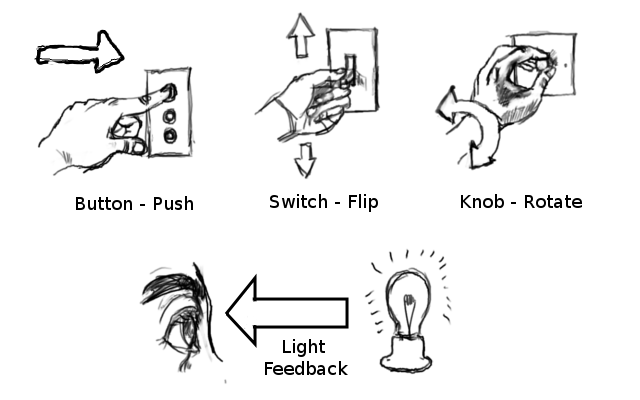
\includegraphics[scale=0.3]{switches.png}
	\end{figure}
\end{frame}

\begin{frame}{Natural mapping}
	\begin{block}{Natural mapping}
	The proper and natural arrangements for the relations between controls and their 	movements to the outcome from such action into the world.
	%The real function of natural mappings is to reduce the need for any information 	from a user’s memory to perform a task.
	\end{block}
	\begin{figure}[ht]
	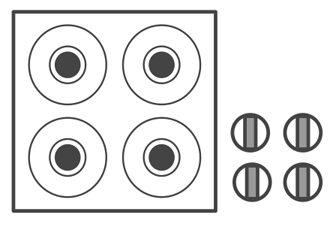
\includegraphics[scale=0.3]{stove_natural.png}
	\end{figure}
	\end{frame}

\begin{frame}{Feedback}
	\begin{block}{Feedback}
	Sending back to the user information about what action has actually been done, what result has been accomplished.
	\end{block}
	\begin{figure}[ht]
	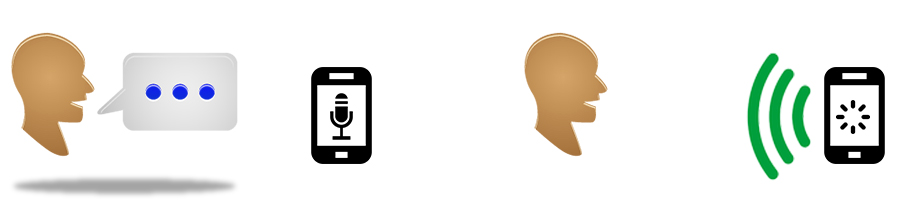
\includegraphics[scale=0.3]{retro-action-speaking.jpg}
	\end{figure}
\end{frame}

\begin{frame}{Logical constraints}
    \begin{itemize}
    		\item User-friendliness
    		\item Call to the human good-sense
            \item Can be induced by natural mapping
    		\item Car windows switches
    \end{itemize}
     \begin{figure}
             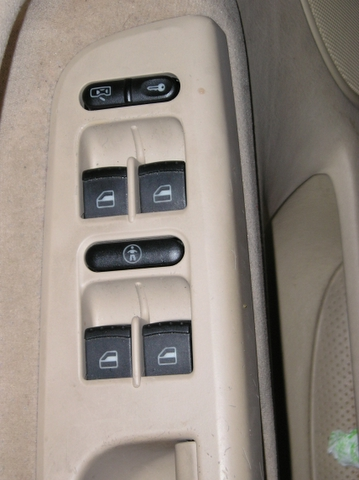
\includegraphics[scale=0.25]{window.jpg}
             \end{figure}
\end{frame}

\begin{frame}{Physical constraints}
    %Left switch for the left lights in a room%
    		 \begin{itemize}
    		 \item Strongest constraints
    		 \item Constrained by physical laws
    		 \item Toolbox
    		 \end{itemize}
             \begin{figure}
             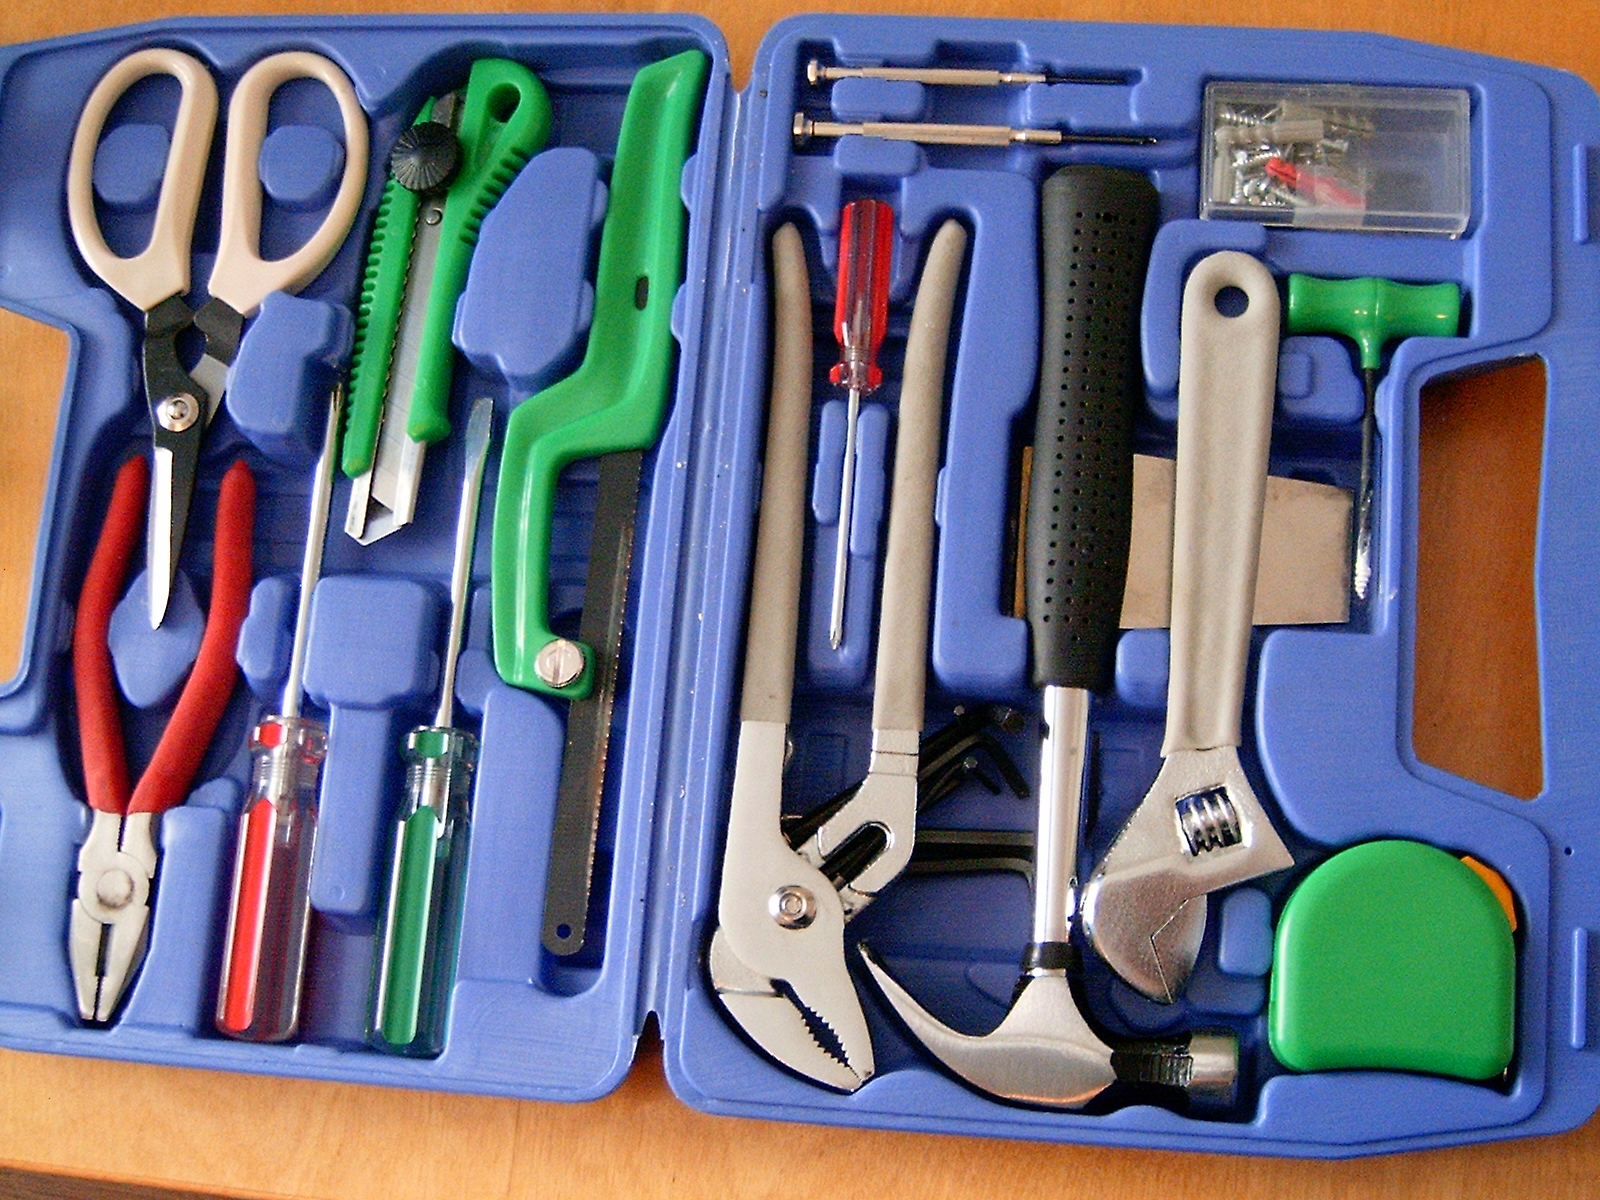
\includegraphics[scale=0.1]{toolbox.jpg}
             \end{figure}

	%Flat key in a flat keyhole%
\end{frame}

\begin{frame}{Cultural constraints}
    \begin{itemize}
		\item Long term learning
    		\item Known situations that can be replicated
    		\item Not universal
    \end{itemize}
    \begin{figure}[ht]
    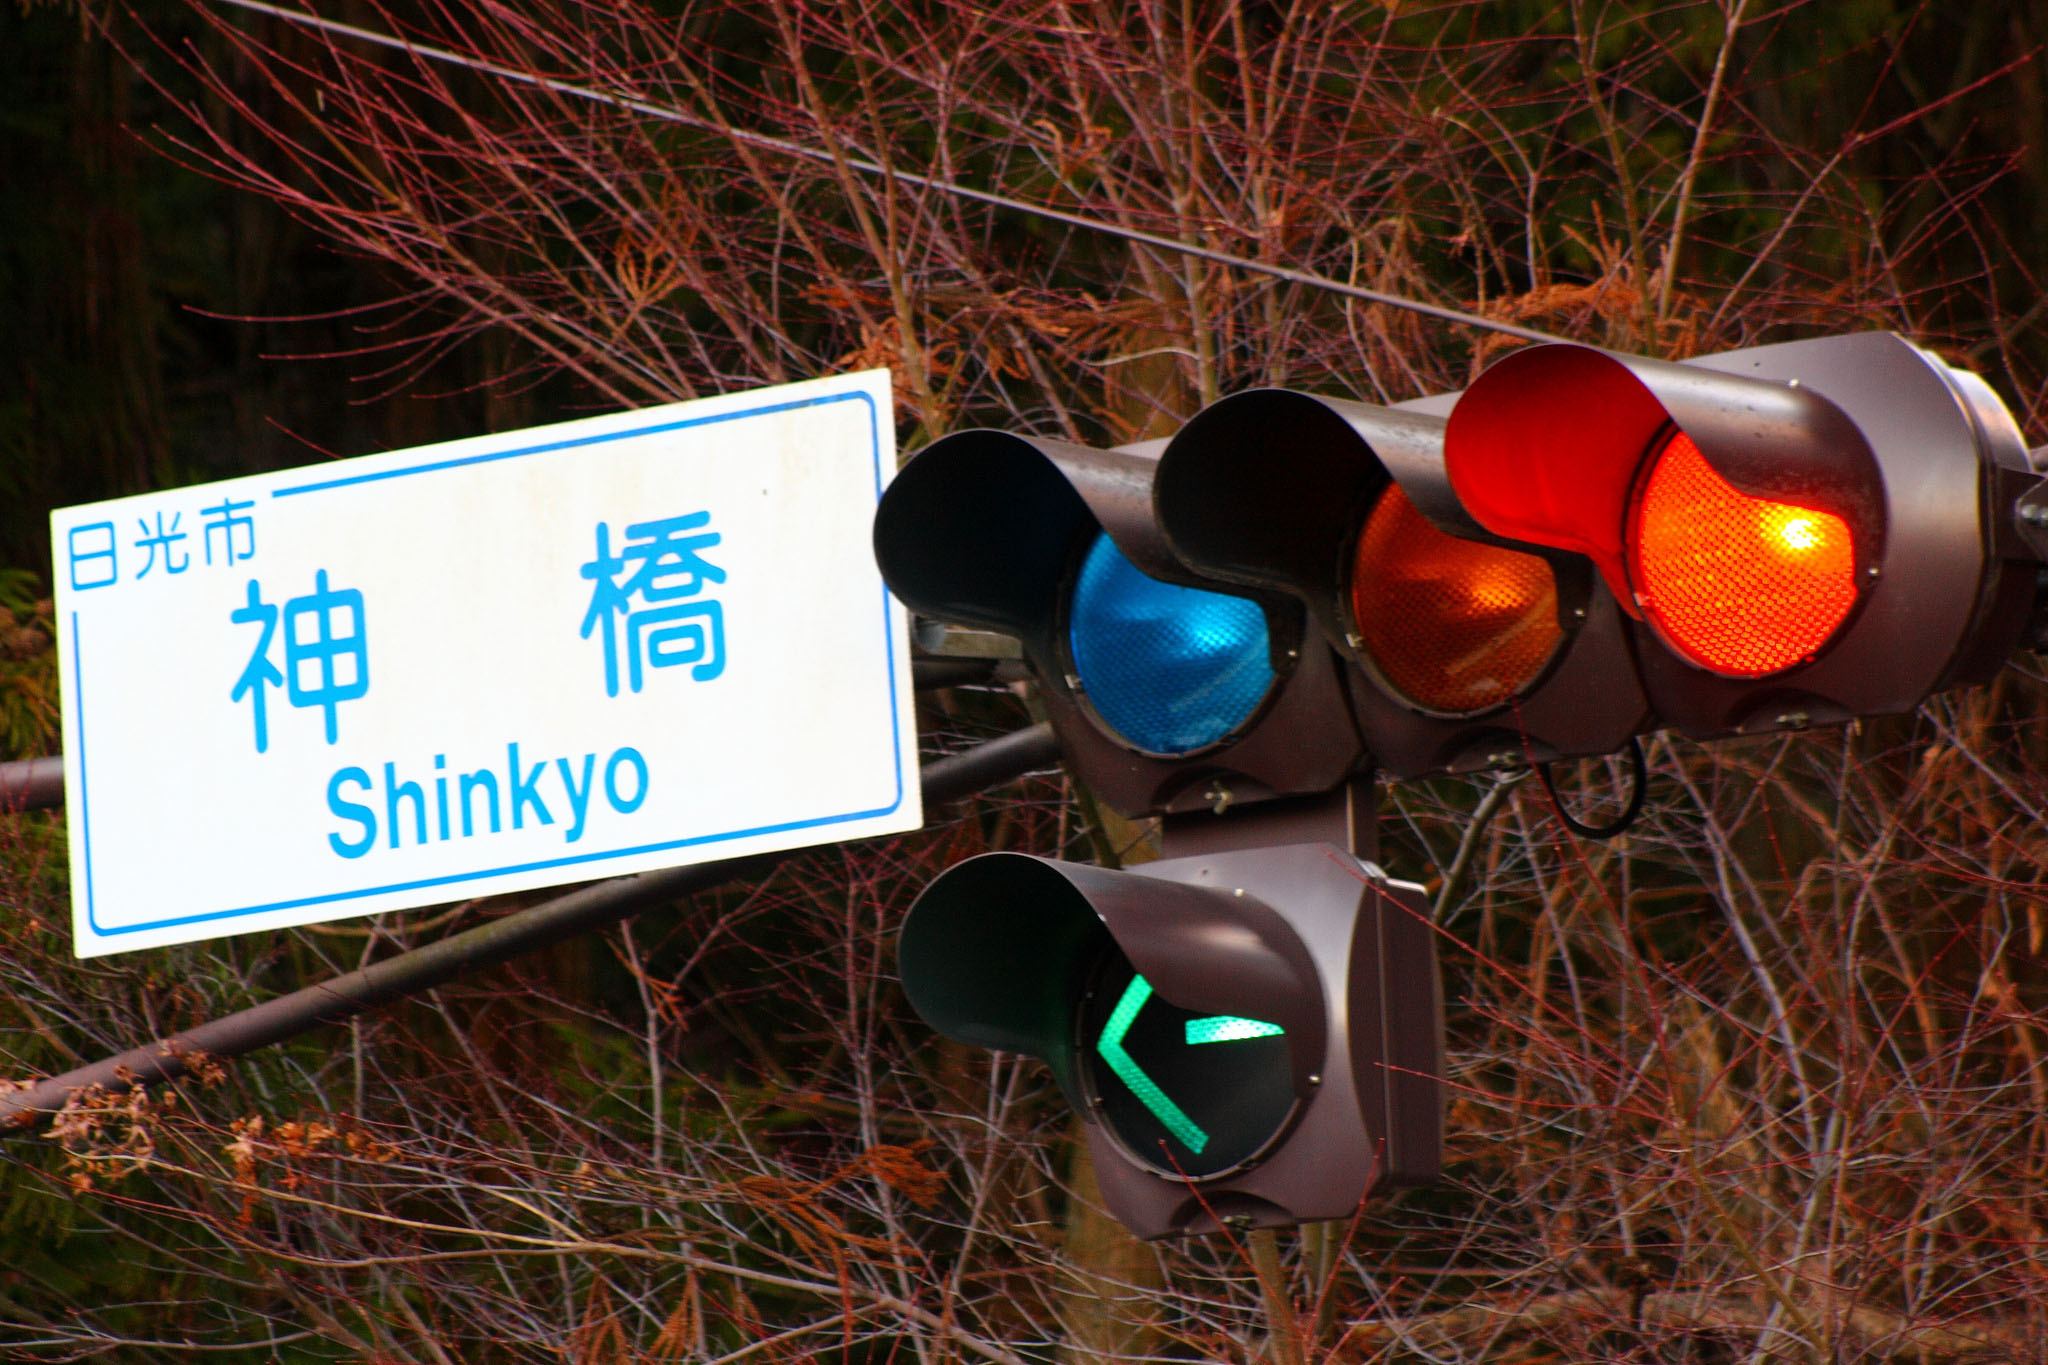
\includegraphics[scale=0.1]{japan-traffic-light.jpg}
    \end{figure}
\end{frame}

\begin{frame}{Semantic constraints}
    \begin{itemize}
    \item Impossible at first try
    \item Short term learning
    \end{itemize}
    \begin{figure}
    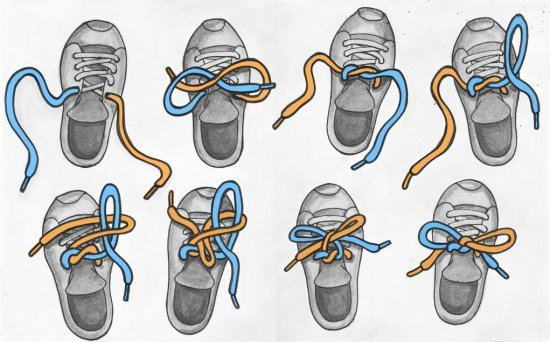
\includegraphics[scale=0.4]{tie_your_shoes.jpg}
    \end{figure}
\end{frame}

\subsection{History of IT design}

\begin{frame}{Outline}
    \tableofcontents[currentsection, currentsubsection]
\end{frame}

\begin{frame}{Evolution in IT:Timeline}

\begin{enumerate}
\item \textbf{1920} Concept of vocal interface: Radio rex
\item \textbf{1960$\rightarrow$1965} Command line interface invention
\item \textbf{1963} Invention of the mouse
\item \textbf{1965$\rightarrow$1985} Massive utilization of CLI
\item \textbf{1970} Neural activity study on monkeys
\item \textbf{1973} First utilisation of a touchscreen (CERN)
\item \textbf{1980 $\rightarrow$ now} Utilization of graphical interface
\item \textbf{early 1980's} Standardization of the mouse
\item \textbf{1983} First commercialized touchscreen computer (by HP)
\item \textbf{1990's $\rightarrow$ now} Standardization of touch interface(e.g PDA)
\item \textbf{end of 1990's $\rightarrow$ now} Standardization of vocal interface(e.g Dragon naturally speaking)
\item \textbf{2000} First proving results of neural interface
\end{enumerate}
\end{frame}

\begin{frame}{Evolution in IT: Command Line Interface}

\begin{itemize}
\item First attempt at design
\item Keyboard: labeled buttons (logical constraint)
\item Basic feedback
\item Lack of affordance
\end{itemize}
	\begin{figure}
			  \begin{minipage}{5cm}
				  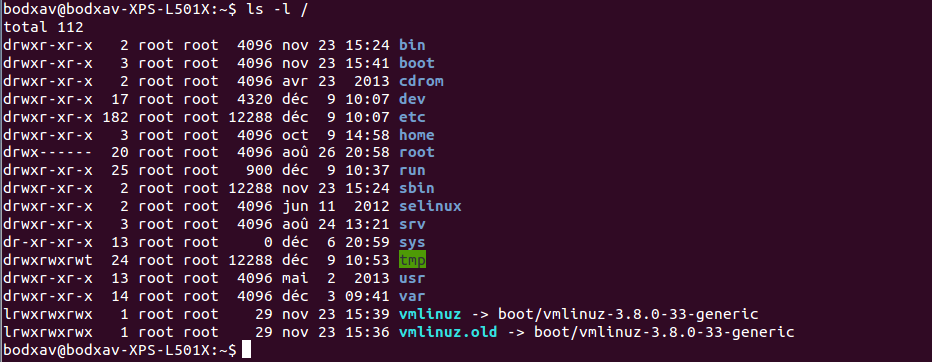
\includegraphics[width=8cm]{terminal.png}
			  \end{minipage}

		\end{figure}
\end{frame}

\begin{frame}{Evolution in IT: Mouse and Graphical User Interface}
\begin{itemize}
\item Invented by Xerox and standardized by Apple
\item Simpler conceptual model: the user interacts with the screen
\item Gain of affordance + natural mapping + feedback
\end{itemize}

\begin{figure}
\raggedleft
	   \begin{minipage}{5cm}
				  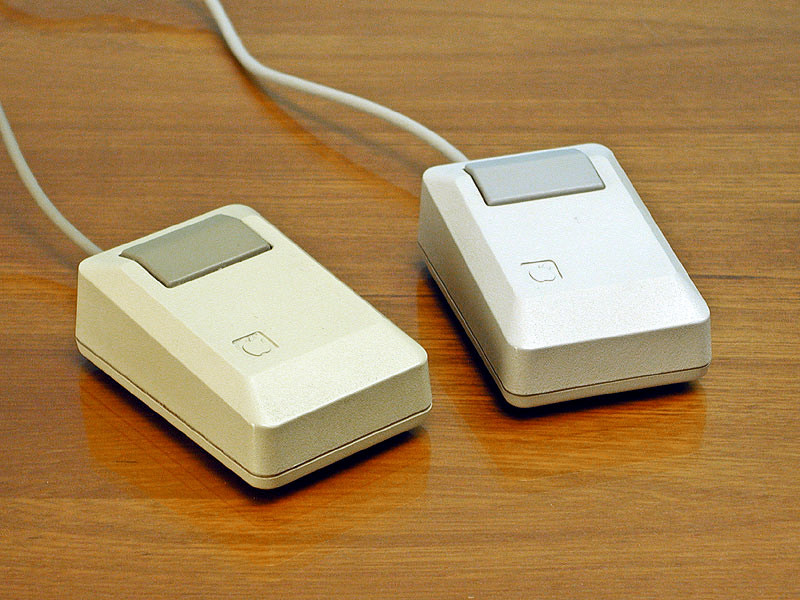
\includegraphics[width=3cm]{mice.jpg}
			  \end{minipage}
			  	   \begin{minipage}{5cm}
				  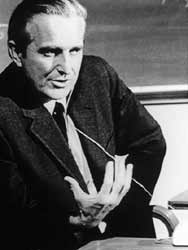
\includegraphics[width=2cm]{doug.jpg}
			  \end{minipage}
\end{figure}
\end{frame}

\begin{frame}{Evolution in IT: Touch interface}
\begin{itemize}
\item Natural affordance: direct interaction with the screen
\item Even simpler conceptual model
\item Complex operations using multiple finger
\item But...
    \begin{itemize}
        \item Less precise than a mouse
        \item Artificial feel
        \item Lack of physical feedback
    \end{itemize}
\end{itemize}
\begin{figure}[ht]
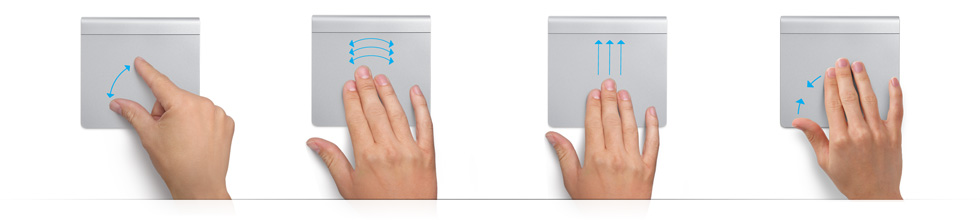
\includegraphics[scale=0.3]{multitouch_gestures_trackpad_2.jpg}
\end{figure}
\end{frame}

\begin{frame}{Evolution in IT: Vocal interface}
\begin{itemize}
\item Very early implementations
\item Closely linked to technology
\item Conceptual model: ask the computer anything
\item In practice: not usable yet
\end{itemize}
\begin{figure}[ht]
\begin{minipage}[b]{0.30\linewidth}
\centering
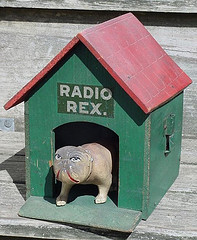
\includegraphics[width=\textwidth]{radio-rex.jpg}


\end{minipage}
\hspace{0.15cm}
\begin{minipage}[b]{0.40\linewidth}
\centering
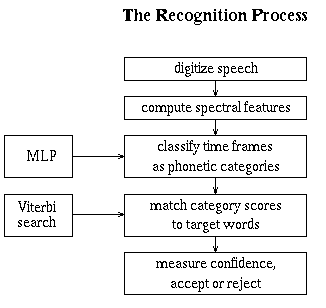
\includegraphics[width=\textwidth]{recognition-process.png}

\end{minipage}
\end{figure}
\end{frame}

\begin{frame}{Evolution in IT : Neuronal interface}
\begin{itemize}
\item Expensive (Still in research)
\item Invasive or Non-invasive interface
\item Matt Nagle case
\end{itemize}

~\\

\begin{center}
    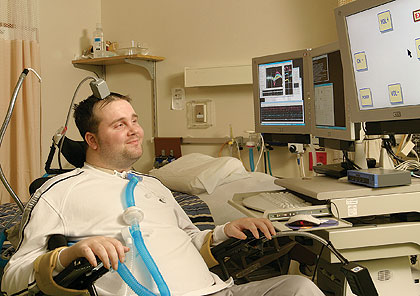
\includegraphics[width=0.4\textwidth]{matt-nagle.jpg} ~
    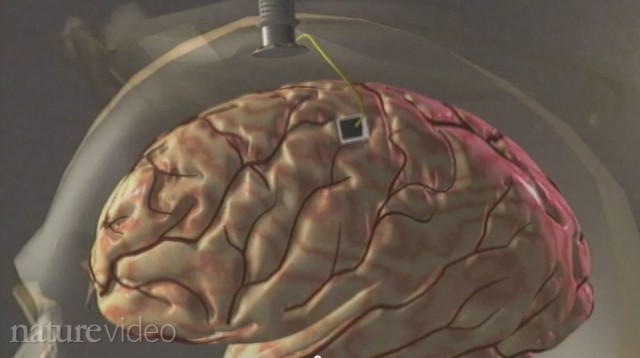
\includegraphics[width=0.4\textwidth]{brain-chip.jpg}
\end{center}

\end{frame}

\subsection{Touchscreen interface: Flat vs. Skeuomorphism}

\begin{frame}{Outline}
    \tableofcontents[currentsection, currentsubsection]
\end{frame}

\begin{frame}{Skeuomorphism}
\begin{block}{Skeuomorph}
An object or feature which imitates the design of a similar artefact made from another material.
\end{block}
\begin{itemize}
\item Skeuos: $\sigma \kappa \varepsilon \upsilon {\rm o} \zeta$ = Tool(or container)
\item Morphê: $\mu {\rm o} \rho \varphi \eta$ = shape
\item Applied to physical and computer/mobile interfaces
\end{itemize}
    \begin{figure}
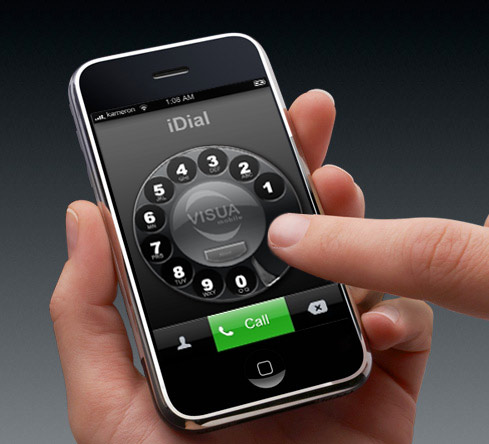
\includegraphics[scale=0.25]{idial.jpg}
\end{figure}


\end{frame}
\begin{frame}{Flat design}
\begin{block}{Flat design}
Flat design is a minimalistic design approach that emphasizes usability. It features clean, open, crisp edges, bright colours and two-dimensional/flat illustrations.
\end{block}
\begin{figure}
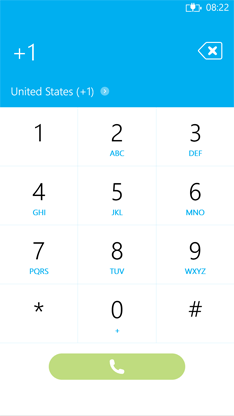
\includegraphics[scale=0.35]{dial-flat.png}
\end{figure}

\end{frame}

\begin{frame}{Comparison}
    \begin{columns}[c]
        \column{.5\textwidth}
            Skeuomorphism
            \begin{itemize}
                \item Intuitive conceptual model
                \item Sense of familiarity
                \item Limited by previous design
            \end{itemize}
        \column{.5\textwidth}
            Flat
            \begin{itemize}
                \item Clean look
                \item Spatially efficient
                \item Cannot rely on previous designs
            \end{itemize}
    \end{columns}
    \begin{columns}[c]
                \column{.5\textwidth}
                    \begin{center}
                    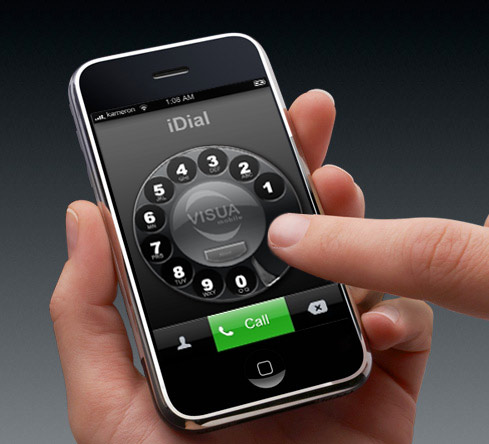
\includegraphics[width=0.7\textwidth]{idial.jpg}
                    \end{center}
                \column{.5\textwidth}
                    \begin{center}
                    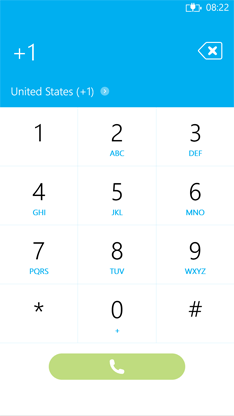
\includegraphics[width=0.4\textwidth]{dial-flat.png}
                    \end{center}
    \end{columns}
\end{frame}

\section{Experimentation}

\begin{frame}{Outline}

	\tableofcontents[currentsection]

\end{frame}

\subsection{Definition of the experiment}
\begin{frame}{Experiment - definition}

\begin{itemize}
    \item We compared two different calculator apps on iPad.
    \item After a short demo of each application, a group of 10 subjects were asked to perform daily tasks with them.
\end{itemize}

\begin{columns}[c]
    \column{.5\textwidth}
        \begin{center}
        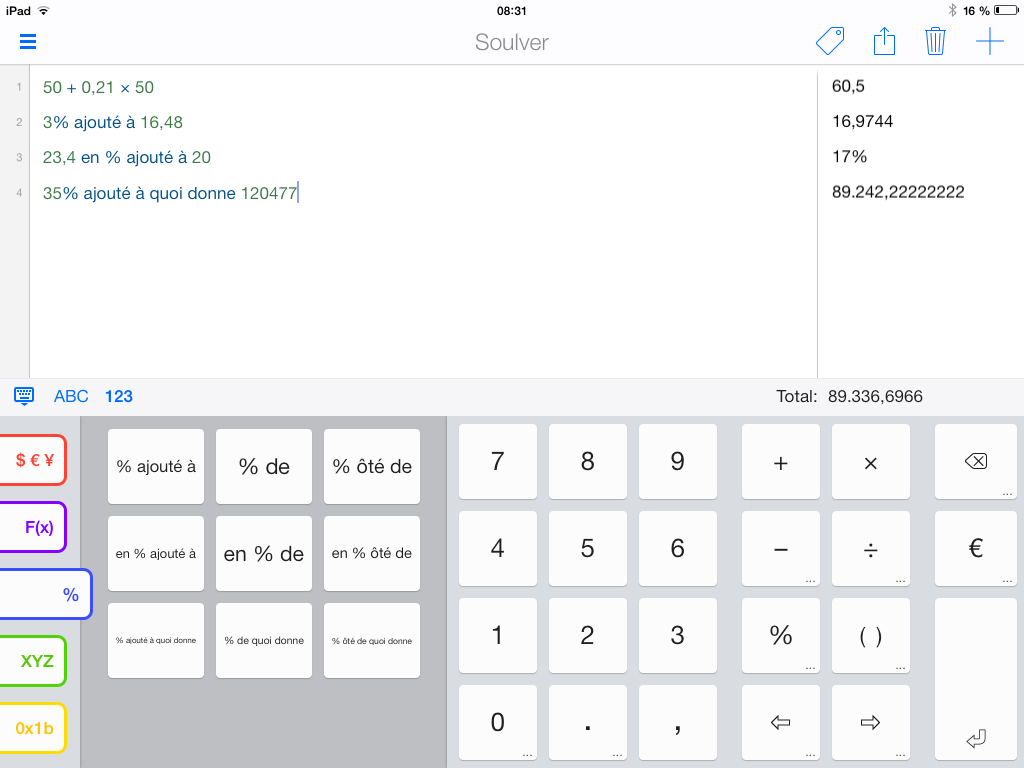
\includegraphics[height=.75\textwidth]{soulveur-screen.png}\\
        Soulver - a flat calculator
        \end{center}
    \column{.5\textwidth}
       \begin{center}
        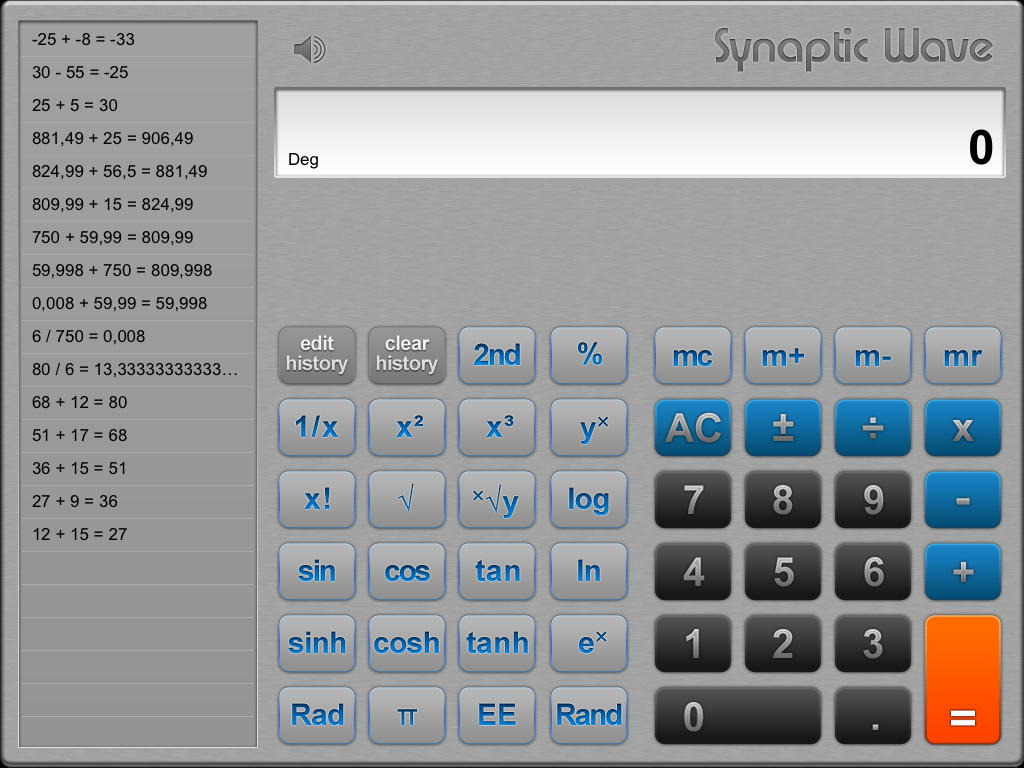
\includegraphics[height=.75\textwidth]{m38-screen.png}\\
        m48+ Emulator
        \end{center}
    \end{columns}

\end{frame}

\subsection{Results}

\begin{frame}{Results - Traveling bill}

    \begin{block}{Instructions}
        Given various bills, calculate expenses made during a trip
    \end{block}

    \begin{itemize}
        \item Most subjects choose Skeuomorphic calculator
        \item Most subjects arrive at the correct result
        \item When asked additional question, subjects were lost
    \end{itemize}

\end{frame}

\begin{frame}{Results - Tax application}

    \begin{block}{Instructions}
        Apply additional tax (in \%) to prices, or find the tax value.
    \end{block}

    \begin{itemize}
        \item We forced subjects to use the other app.
        \item Soulver has dedicated functions for percentage, but they were rarely used
        \item Subjects rarely got the correct result
    \end{itemize}

\end{frame}

\begin{frame}{Results - Debriefing}
    \begin{block}{Instructions}
        What are your thought on each app?
    \end{block}

    \begin{itemize}
        \item bli
        \item blo
        \item blu
    \end{itemize}
\end{frame}


\section{Previous results}
\subsection{Flat VS Skeuomorph icons (June 2013)}

\begin{frame}{Outline}
    \tableofcontents[currentsection]
\end{frame}

\begin{frame}{Flat VS Skeuomorph icons}
	\begin{figure}
	\centering
	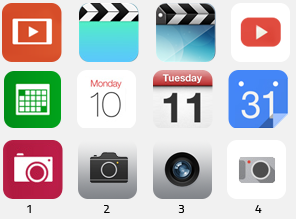
\includegraphics[scale=0.5]{flat.png}
	\end{figure}
    \begin{center}
      \begin{tabular}{|l|c|c|c|c|}
        \hline
        &Windows 8 & IOS7 & IOS6 & Google\\
        \hline
        Video App 	& 19\%	& 22\%	& 21\%	& 38\% \\
        Calendar App& 10\%	& 44\%	& 23\%	& 23\% \\
        Video App	& 24\%	& 22\%	& 30\%	& 24\% \\
        \hline
        Average		& 17.6\%& 29.3\%& 24.6\%& 28.3\% \\
        \hline
      \end{tabular}
    \end{center}
    	\begin{flushright}\tiny\url{www.grapheine/divers/flat-design-vs-skeumorphisme}\normalsize\end{flushright}
\end{frame}

\subsection{Windows survey (Sept 2012)}
\begin{frame}{Windows survey about new users of windows 8}

    \small
    \begin{center}
      \begin{tabular}{|l|c|c|c|c|}
        \hline
        & Windows 8 & Windows 7 & Windows XP & Others\\
        \hline
        Already used windows & 26\%	& 75\%	& 58\%	& 17\% \\
        Prefered windows	 & 25\%	& 53\%	& 20\%	& 2\% \\
        \hline
      \end{tabular}
    \end{center}
    \normalsize
    \begin{columns}[c]
      \column{.5\textwidth}
      \begin{figure}
        \centering
        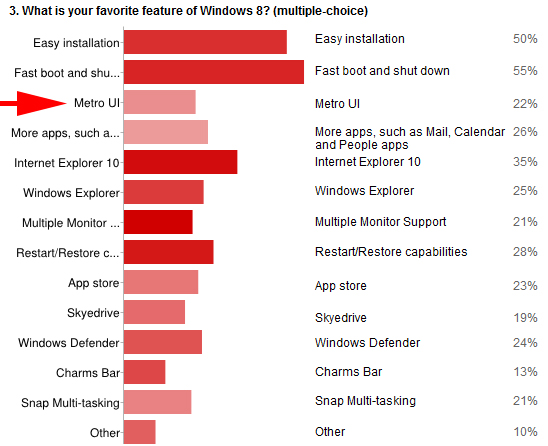
\includegraphics[scale=0.25]{windows8UI.jpg}
      \end{figure}
      \column{.5\textwidth}
      \begin{figure}
        \centering
        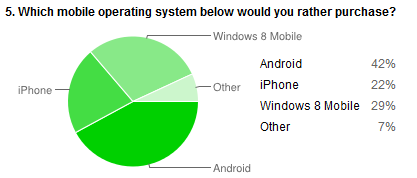
\includegraphics[scale=0.25]{windows8Phone.png}

        \centering
        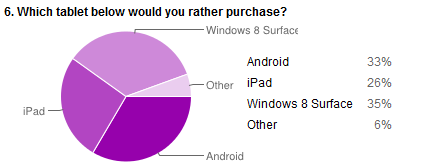
\includegraphics[scale=0.25]{windows8Tablet.png}
      \end{figure}

	\end{columns}
	\begin{flushright}\tiny\url{www.forumswindows8.com/general-discussion/windows-8-survey-half-prefer-windows-7-a-7853.htm}\normalsize\end{flushright}
\end{frame}



\subsection{Japanese study about concrete and flat design (March 2013)}
\begin{frame}{Japanese study about concrete and flat design}
	\begin{itemize}
    \item Vast choice of app, first impression is important. Design of the icon should be well choosen\\
    \begin{figure}
        \centering
        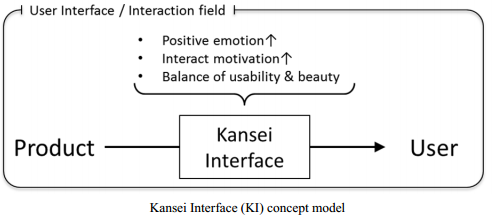
\includegraphics[scale=0.5]{UI.png}
      \end{figure}
    \item Icons analysed by 8 designers with one questionnaire, and by 42 buyers of apps with another. Tried to find best correlation between particularities to make a map
    \end{itemize}
	\begin{flushright}\tiny\url{http://design-cu.jp/iasdr2013/papers/1811-1b.pdf}\normalsize\end{flushright}
\end{frame}

\begin{frame}{Japanese study about concrete and flat design (2)}
    \begin{figure}
        \centering
        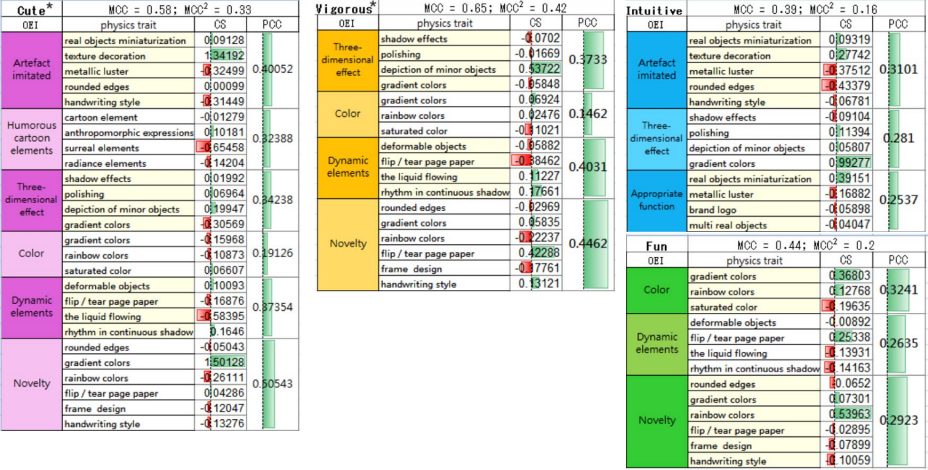
\includegraphics[scale=0.45]{caract.png}
      \end{figure}
	\begin{flushright}\tiny\url{http://design-cu.jp/iasdr2013/papers/1811-1b.pdf}\normalsize\end{flushright}
\end{frame}

\begin{frame}{Japanese study about concrete and flat design (3)}
	\begin{columns}[c]
      \column{.6\textwidth}
      \begin{figure}
        \centering
        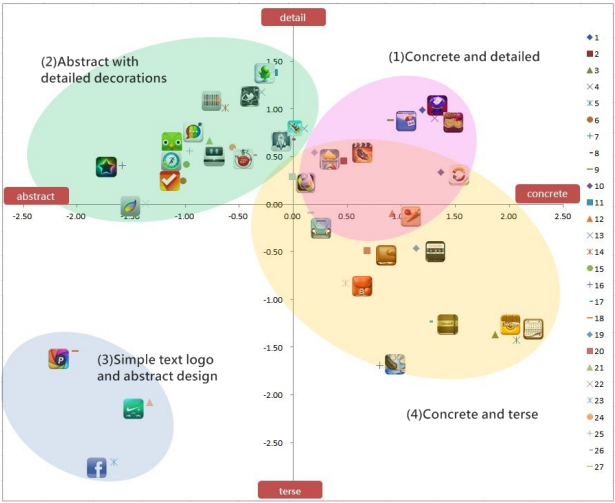
\includegraphics[scale=0.45]{map.png}
      \end{figure}
      \column{.4\textwidth}
      \begin{itemize}
        \item Preference between 16 icons
        \item 77 participants
        \item 77\% smartphones
        \item 23\% featurephones
      \end{itemize}
	\end{columns}
	\begin{flushright}\tiny\url{http://design-cu.jp/iasdr2013/papers/1811-1b.pdf}\normalsize\end{flushright}
\end{frame}

\begin{frame}{Japanese study about concrete and flat design (4)}
	\begin{figure}
    	\centering
        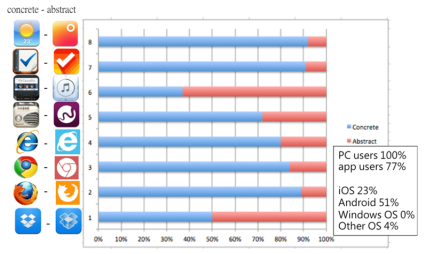
\includegraphics[scale=0.6]{finalStat.png}
    \end{figure}
    \begin{itemize}
        \item 75\% prefer concrete icons
		\item Icon music is different... Old item not used anymore?
    \end{itemize}
	\begin{flushright}\tiny\url{http://design-cu.jp/iasdr2013/papers/1811-1b.pdf}\normalsize\end{flushright}
\end{frame}

%\bibliographystyle{amsalpha}
%\bibliography{dit-paper}

\end{document}
